\section{惯性 惯性的应用}\label{sec:3-7}

我们从牛顿第一运动定律知道,物体有保持匀速直线运动状态或静止状态的性质。这个性质是任何物体都具有的。
我们\CJKunderwave{把物体保持匀速直线运动状态或静止状态的这种性质叫做惯性}。
因此牛顿第一运动定律也常常叫做\textbf{惯性定律}。

一切物体都有惯性。表现物体惯性的现象是经常可以遇到的。我们把钢球放在硬纸片上(图 \ref{fig:3-6})。
把硬纸片突然弹出去,钢球由于惯性要保持原来的静止状态,所以仍然留在原处,掉进筒里;
当火车或汽车突然开动的时候,乘客会倒向跟车行相反的方向,也是这个道理。

\begin{figure}[htbp]
    \centering
    \begin{minipage}{4cm}
    \centering
    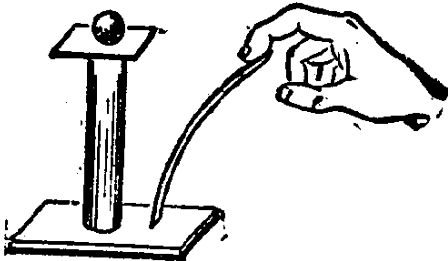
\includegraphics[width=4cm]{../pic/czwl1-ch3-6}
    \caption{}\label{fig:3-6}
    \end{minipage}
    \qquad
    \begin{minipage}{10cm}
    \centering
    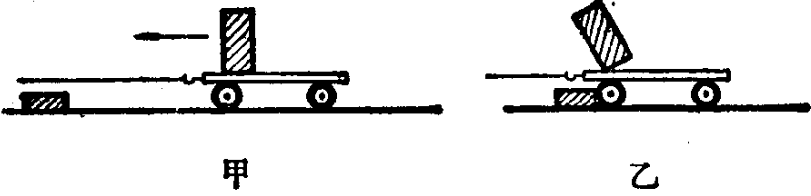
\includegraphics[width=10cm]{../pic/czwl1-ch3-7}
    \caption{}\label{fig:3-7}
    \end{minipage}
\end{figure}



把一个木块直立在小车上,让小车沿着桌面运动( 图 \ref{fig:3-7} 甲)。当小车遇到障碍物而突然停止的时候,
车上的木块就向前面倒下( 图 \ref{fig:3-7} 乙) 。小车突然停止的时候,由于木块和车面之间的摩擦,
木块的底部也随着停止,可是木块的上部由于惯性要保持原来的运动状态,仍然继续前进,所以木块倒向前方。
我们奔跑的时候,脚碰在障碍物上就会跌向前方;当火车或汽车突然停止的时候,乘客会倒向车行的方向,都是同样的道理。

惯性的应用是很多的,锤头松了,把锤柄的一端在固定物体上撞击几下,锤柄因撞击而突然停止,
锤头由于惯性仍然要继续前进,结果就紧套在锤柄上了。射击的时候,子弹在枪膛里受到火药气体的推力获得很大速度,
离开枪口后不再受到火药气体的推力,但是子弹由于惯性,仍然继续高速前进,击中远处目标。
物体的惯性对我们也有不利的一面。行驶中的汽车或火车,由于惯性不能立刻停止。
即使紧急刹车,也要向前运动一段距离才能停下来。


\lianxi

(1) 请一位骑自行车的同学握着一块石头从你面前驶过,并且刚好在驶到你面前的瞬间放开手,让石头自由落下。
观察石头落在哪里。说明石头为什么不是落在你面前的地上,而如果自行车停在你面前不动石头无疑是会那样的。

(2) 飞机投殚,不是在飞到目标的正上方时投掷,而是要提前投掷,才能命中目标,为什么?

(3) 烧锅炉的时候,用铲子送煤,铲子往往并不进入灶内,而是停在灶前,煤就顺着铲子运动的方向进入灶内,为什么?

(4) 为什么从行驶的车上跳下来容易摔倒?

(5) 把一摞棋子放在桌上,用一根薄木条贴着桌面迅速打击底下的棋子,会看到什么现象?做做看,并解释你看到的现象。

(6) 把一小块石头或砖放在纸条上,尽快抽动纸条,你看到什么现象?你会解释这个现象吗?

(7) 举出几个你在生活和生产中应用惯性的例子。


